%*******************************************************************************
%****************************** Second Chapter *********************************
%*******************************************************************************

\chapter{Imaging focus: the microfludics environment}

\ifpdf
    \graphicspath{{Chapter2/Figs/Raster/}{Chapter2/Figs/PDF/}{Chapter2/Figs/}}
\else
    \graphicspath{{Chapter2/Figs/Vector/}{Chapter2/Figs/}}
\fi

%********************************** %First Section  **************************************
\section{Purpose and the need for segmentation}

The reason this environment was developed is to determine how cancer cells cross the endothelium (blood vessel wall cell barrier) during extravasation, or the stage of metastasis where cancerous cells that have already entered the blood stream from some initial location, make their way around the body, break through the blood vessel wall, and embed themselves in another type of tissue. Extravasation is a partially understood process in cancer biology~\cite{Reymond:13}, and this type of system could help to understand it by providing accurate data on the morphodynamics of the cells as they move in the simulation of a blood vessel.

To provide useful data, information about a great many cells must be gathered. This requires visually identifying cells and parts of cells and assessing their changing shapes, sizes, and speeds over time and in distinct regions of the environment. This can be done manually by keeping track of each cell and recording its progress over the course of the experiment. Unfortunately, this is impractical for the amount of data needed and would be too time consuming for a human to do. As such, it must be done automatically. This type of recognition done by a computer is known as segmentation, where cell shapes are separated and differentiated from the background. Many algorithms, techniques, and pieces of software exist to solve this with varying levels of success. They require a mathematical description of a set of images, and a way to consistently find features of the objects of interest that can be matched and measured.

Certain aspects of the environment used in the experiment and the methods by which it was imaged pose problems for accurate cell segmentation by disrupting the consistency that cell segmentation algorithms depend on. Traditional cell microscopy using glass slides and chemically fixed cells allows for high resolution images of cells that are consistently in focus. Factors affecting the quality in this case are the 3D structure of the channel, the live cell environment where cells are free to move and interact, and the movement of the microscope hardware and cancer cells vertically (relative to the microscope objective) that causes object to fluctuate in and out of focus in the final data.

\section{Confocal microscope and 3D structure}

Image data were gathered using a confocal microscope. This allows a 3D space to be imaged by scanning over a volume and recording data at a number of discreet levels. Data can also be recorded in a number of different channels (the brightfield channel is shown below in Figure~\ref{fig:sampleimagedata}). The data for these experiments used brightfield, or transmission, images and GFP fluorescence images. The light in brightfield images from different levels is mixed (blurred) by the optics of the microscope objective, resulting in distorted representations of objects unless their level is in focus. In contrast, light from GFP inside cells can be isolated to a particular level using the pinhole mechanism of the microscope. The size of the pinhole determines the maximum resolution of the image. This isolation of the GFP channel levels can be used to build up a 3D model of the objects marked with GFP, which in this experiment is only the cancer cells. Cancer cells can then be distinguished from other types of objects in the experiment.

\begin{figure}[h!]
 \centering
 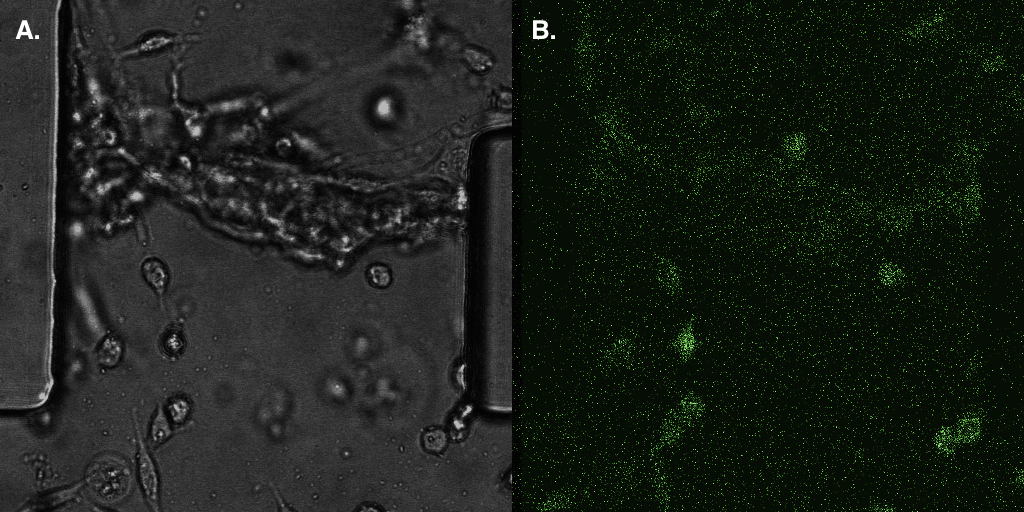
\includegraphics[width=0.9\textwidth]{201_sample_data}
 \caption[Sample image data]{
 	This is sample of image data obtained from the microscope. Each image shows a single slice from a single frame in one series of an experiment. A shows the brightfield image, while B shows the GFP for the corresponding slice. The same physical space is represented by both images. This correspondence can be exploited to make use of useful information from both images.
 }
 \label{fig:sampleimagedata}
\end{figure}

The 3D information from the GFP can be used to locate cancer cells within the environment, but the limits on the resolution prevent accurate outlines of the cells from being found. This is also dependent on the cells' internal distribution of GFP. The cancer cells in the current experiments had GFP embedded within the cytosol, or the fluid interior of the cell. From this, the general bulk of the cell and to a certain extent its general shape could be made out, but finer edges and protrusions could not be determined since the GFP did not penetrate the cytoskeleton or the outer wall of the cell. The method used to find cells and prepare the images for segmentation is directly dependent on the this arrangement of the GFP. modifications can be made to account for other sources of fluorescence inside the cell. This is discussed more in Chapter 3.

\section{Description of the environment}

The microfludics environment used for this study consisted of a microchannel framework printed using soft lithography on a PDMS chip. PDMS, or Polydimethylsiloxane, is a silicone gel that can be molded and used to create microscopic structures, such as microscopic channels to use as environments for cells~\cite{Zheng:10}\cite{Herold:09}\cite{Halldorsson:15}. This microchannel technique is seen as a potentially groundbreaking paradigm in the biomedical industry to mimic body tissue for complex \emph{in vitro} studies. In this case, the channel was set up to model a human blood vessel. The diagram in Figure~\ref{fig:model} below shows part of the channel framework with two PDMS pillars on either side of a gap. On one side of the gap, a liquid medium meant to simulate blood plasma is pumped in where it can remain static, or be used to simulate the flow inside a blood vessel. On the other side of the gap, collagen gel, used to simulate the extracellular matrix surrounding a blood vessel, provides an anchor point for the endothelial cells, or cells found in the blood vessel wall, to attach to. These endothelial cells are added to the environment prior to the experiment. The experiment is monitored when cancer cells that are marked with a fluorescent GFP, or Green Fluorescent Protein, are added to the environment in the medium channel, from which they can cross the endothelial cell barrier into the collagen gel, as they might \emph{in vivo} during the extravasation stage of metastasis~\cite{Reymond:13}.

\begin{figure}[h!]
 \centering
 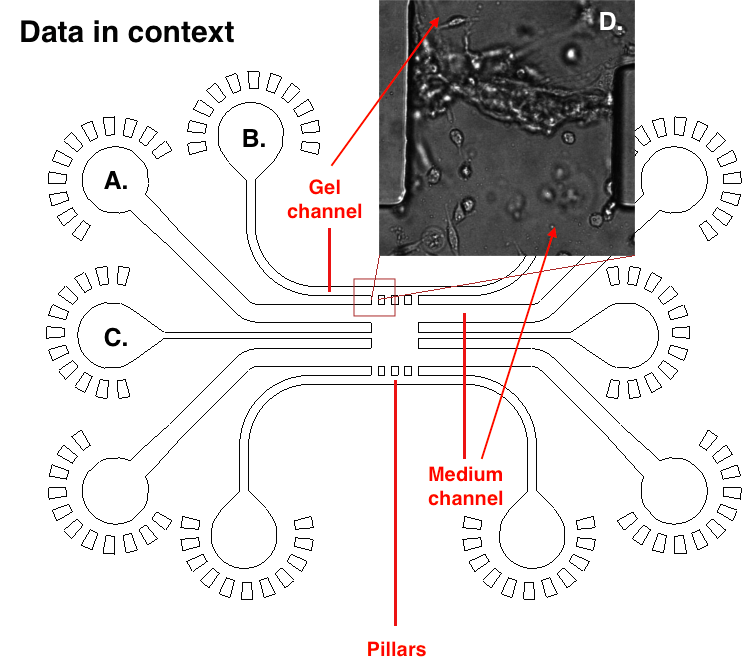
\includegraphics[width=0.9\textwidth]{202_model}
 \caption[Microfludics device and data in context]{
 	This diagram shows a schematic of the microfluidics environment used in the current set of experiments and a small sample of data captured from it. The spread out nodes (a,b) at the ends of the channels are feeds for the channels in the centre of the device. Liquid and cell matter can be placed in these feeds to seed the environment. Feed a) leads to the medium channel adjacent to the pillars. Feed b) leads to the gel channels on the top and bottom of the device. The feed in the centre of the environment is designed to introduce drugs and other chemicals into the medium channel at the point of contact between the gel and medium (the pillars). The image D is the same data as shown in Figure~\ref{fig:sampleimagedata}, but placed in context of the device.
 }
 \label{fig:model}
\end{figure}

The entire channel is approximately 100 microns thick. this is roughly an order of magnitude greater than the width of a typical cancer cell used in the experiments. During the experiment the cells may be attached (flattened) and thus much thinner vertically. The width of the gap horizontally containing the endothelial cell barrier is between 100-200 microns. A typical blood vessel would be tubular, but this setup, while possible, would be difficult to study and to image with a microscope. Opting instead for the simplified setup, the vertical wall of cells can be observed much more easily and still be used to provide information on how the cancer cells cross the barrier. More advanced setups are under development at the time of writing.

\section{Live cell imaging limitations}

Imaging live cells imposes limits on the techniques available since the cells must remain alive and be able to behave naturally for the entire duration of the experiment. This means they cannot be subjected to excess illumination from the laser used to stimulate fluorescence lest they absorb too much energy and overheat, causing erratic movements and finally death, making any data on their movements unusable. This limit on the amount of light that one is able to put into the cells to stimulate the GFP limits the amount of light that can be gathered from the cells. This lowers the brightness and contrast of the final data, making the location of finer details in a cell less certain.

The cells are also free to move about the environment. Tracking a single cell means it must remain in the field of view. The time period in this experiment necessary to allow the cells to cross the endothelial barrier is between 10-15 hours, and the distance a cell can move in this time sets a lower limit on the size of the viewport, or the view of the microscope that is finally recorded as an image. A large viewport means a lower resolution, since the objective must move away from the sample. This sacrifices image quality per cell for information about many cells. For this trade-off to be worthwhile, useful data must be extracted from the lower quality cell images. This is difficult for simple cell segmentation algorithms.

The movement of the cells is not restricted to the two dimensions of the viewport. The cells can move up and down in the environment (towards and away from the objective). This will move them between different focal planes. While all this data is recorded, cells cannot be guaranteed to stay on one level for the whole experiment. As a cell moves vertically, its representation in the image will change and properties of its edges will change their colour and texture. This breaks the feature consistency that segmentation relies on.

\section{Autofocus and focal fluctuations}

Apart from the behaviour of the cells, the microscope hardware must also operate reliably for the 10-15 hour time period. This is not always possible, and small changes in the alignment of different components will cause systematic errors to build up and compound over time. The result of the microscope imaging in one alignment while the instruments report another causes errors in the consistency of the image sequence. The focus will fluctuate visibly while an index representing the focal plane remains the same. This means such an index cannot be relied on the accurately report the location in the environment.

Software that is meant to solve this problem is known as Autofocus~\cite{Firestone:91}. Most commercial microscope setups come with this software preinstalled. It attempts to analyse the images gathered at regular intervals, for example, every frame, and determine the current focal plane in the environment from simple numerical properties. An example of such a property is the minimum entropy of the image~\cite{Firestone:91}. By keeping the minimum entropy constant, the image plane with the most similar entropy in the next frame can be found. This is set as the corresponding level so that representations of the objects remain constant. Other methods such as measuring the reflection of light from the cover slip of the sample are also used~\cite{Poland:08}. Highly variable environments such as live cells can cause misleading calculations of a constant entropy, hence the unreliability of the level index. This makes segmentation more complicated.
